

\section{Hydrogen Production}

    \subsection{Overview Flowsheet}
    \begin{figure}[H]
        \centering
        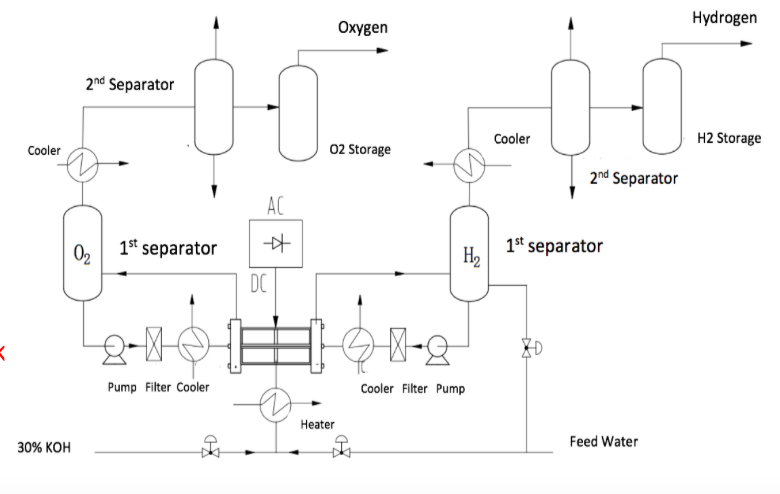
\includegraphics[width=0.87\textwidth]{flowsheet.png}
        \caption{Electrolysis system flowsheet [Slide 18 ]}
        \label{fig:plant_schematic}
    \end{figure}
    
  \subsection{Polarisation Curve}
\begin{figure}[H]
\centering
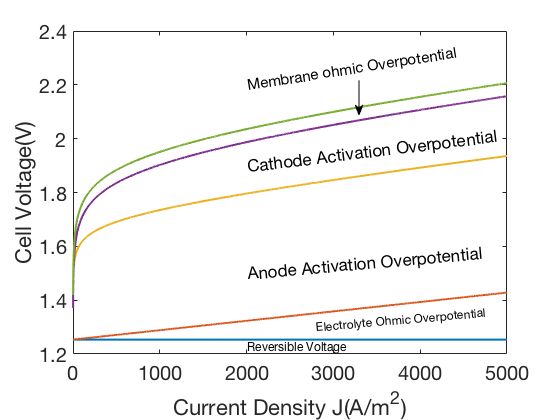
\includegraphics[width=0.7\textwidth]{pres3.png}
\caption{Polarisation curve[Slide 19]} 
\end{figure}    


    
  \subsection{Operating Conditions}
\begin{figure}[H]
\centering
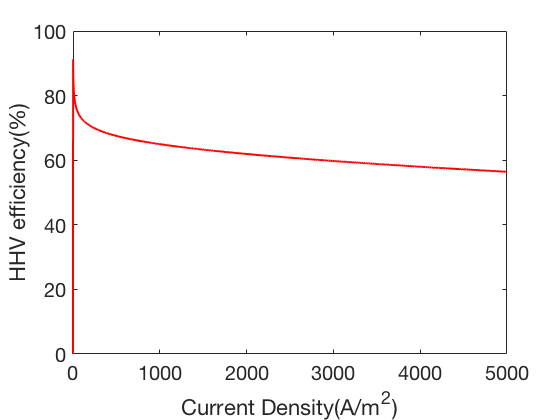
\includegraphics[width=0.45\textwidth]{pres1.png}
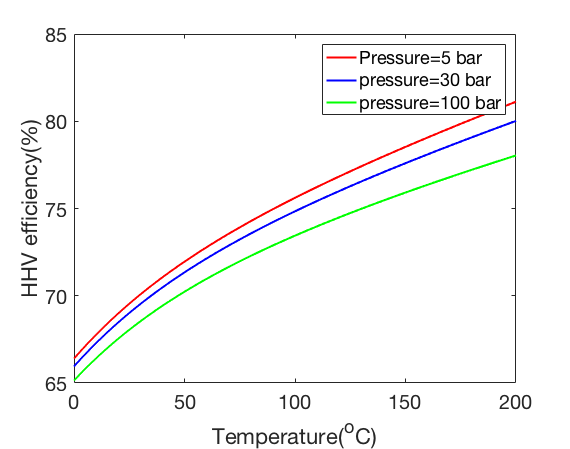
\includegraphics[width=0.45\textwidth]{pres2.png}
\caption{Effects of temperature, pressure and current density on HHV efficiency[Slide 20]} 
\end{figure} 

\subsection{Configuration}
\begin{figure}[H]
\centering
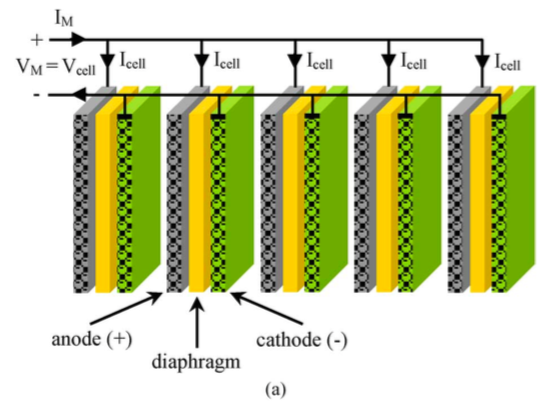
\includegraphics[width=0.55\textwidth]{monopolar.png}
\caption{Monopolar configuration}
\end{figure}
\begin{figure}[H]
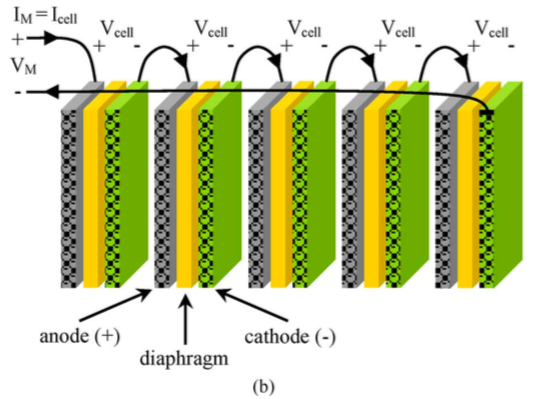
\includegraphics[width=0.55\textwidth]{bipolar.png}
\caption{Bipolar configuration[Slide 21]} 
\end{figure} 


\subsection{Zero-gap configuration}
\begin{figure}[H]
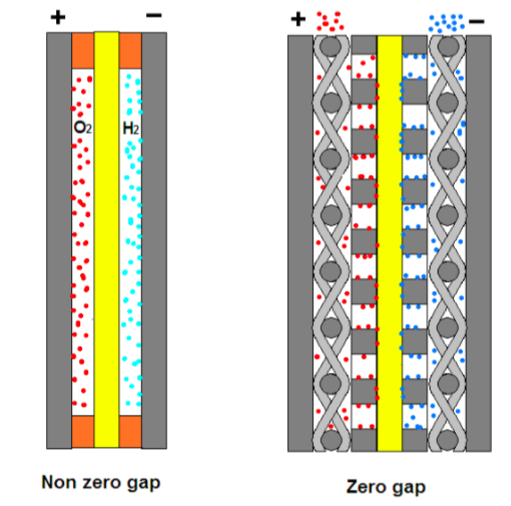
\includegraphics[width=0.30\textwidth]{zerogap.png}
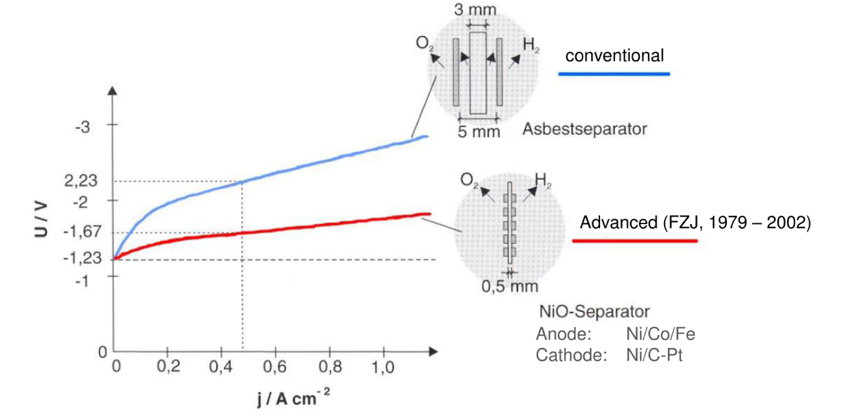
\includegraphics[width=0.55\textwidth]{zerogapgap.png}
\caption{Monopolar and Bipolar configuration[Slide 22]} 
\end{figure} 

\subsection{Electrolyser Control System}
\begin{figure}[H]
\centering
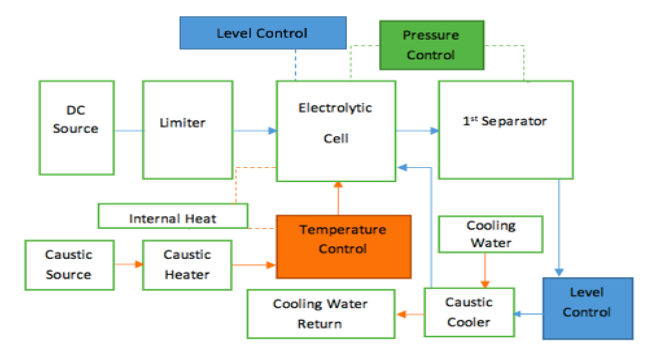
\includegraphics[width=0.70\textwidth]{controlcontrol.png}
\caption{Electrolyser Control System[Slide 24]} 
\end{figure}
\begin{figure}[H]
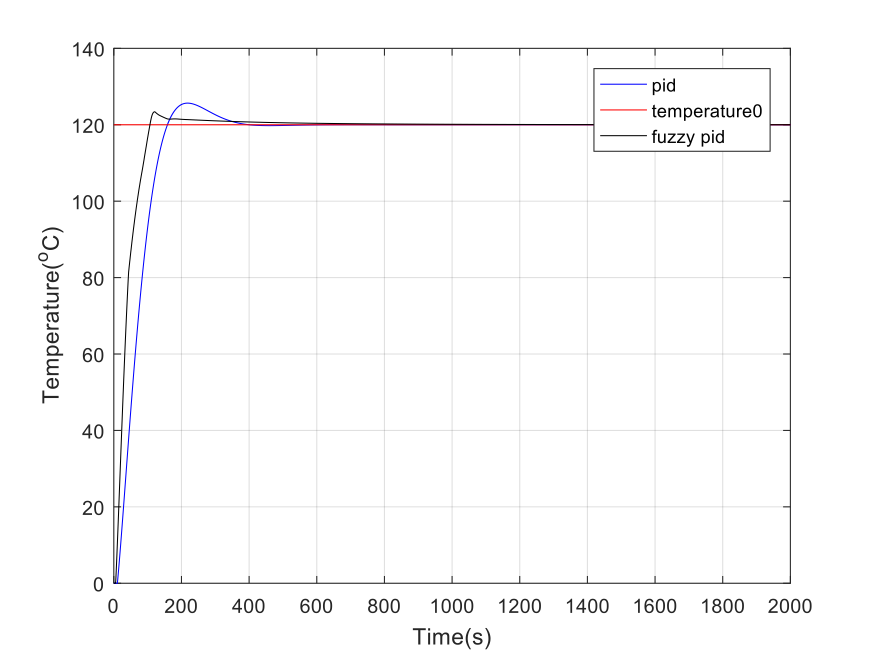
\includegraphics[width=0.50\textwidth]{pidpid.png}
\caption{Fuzzy PID and traditional PID controller comparison[Slide 26]} 
\end{figure} 






\subsection{Simulation}
\begin{figure}[H]
\centering
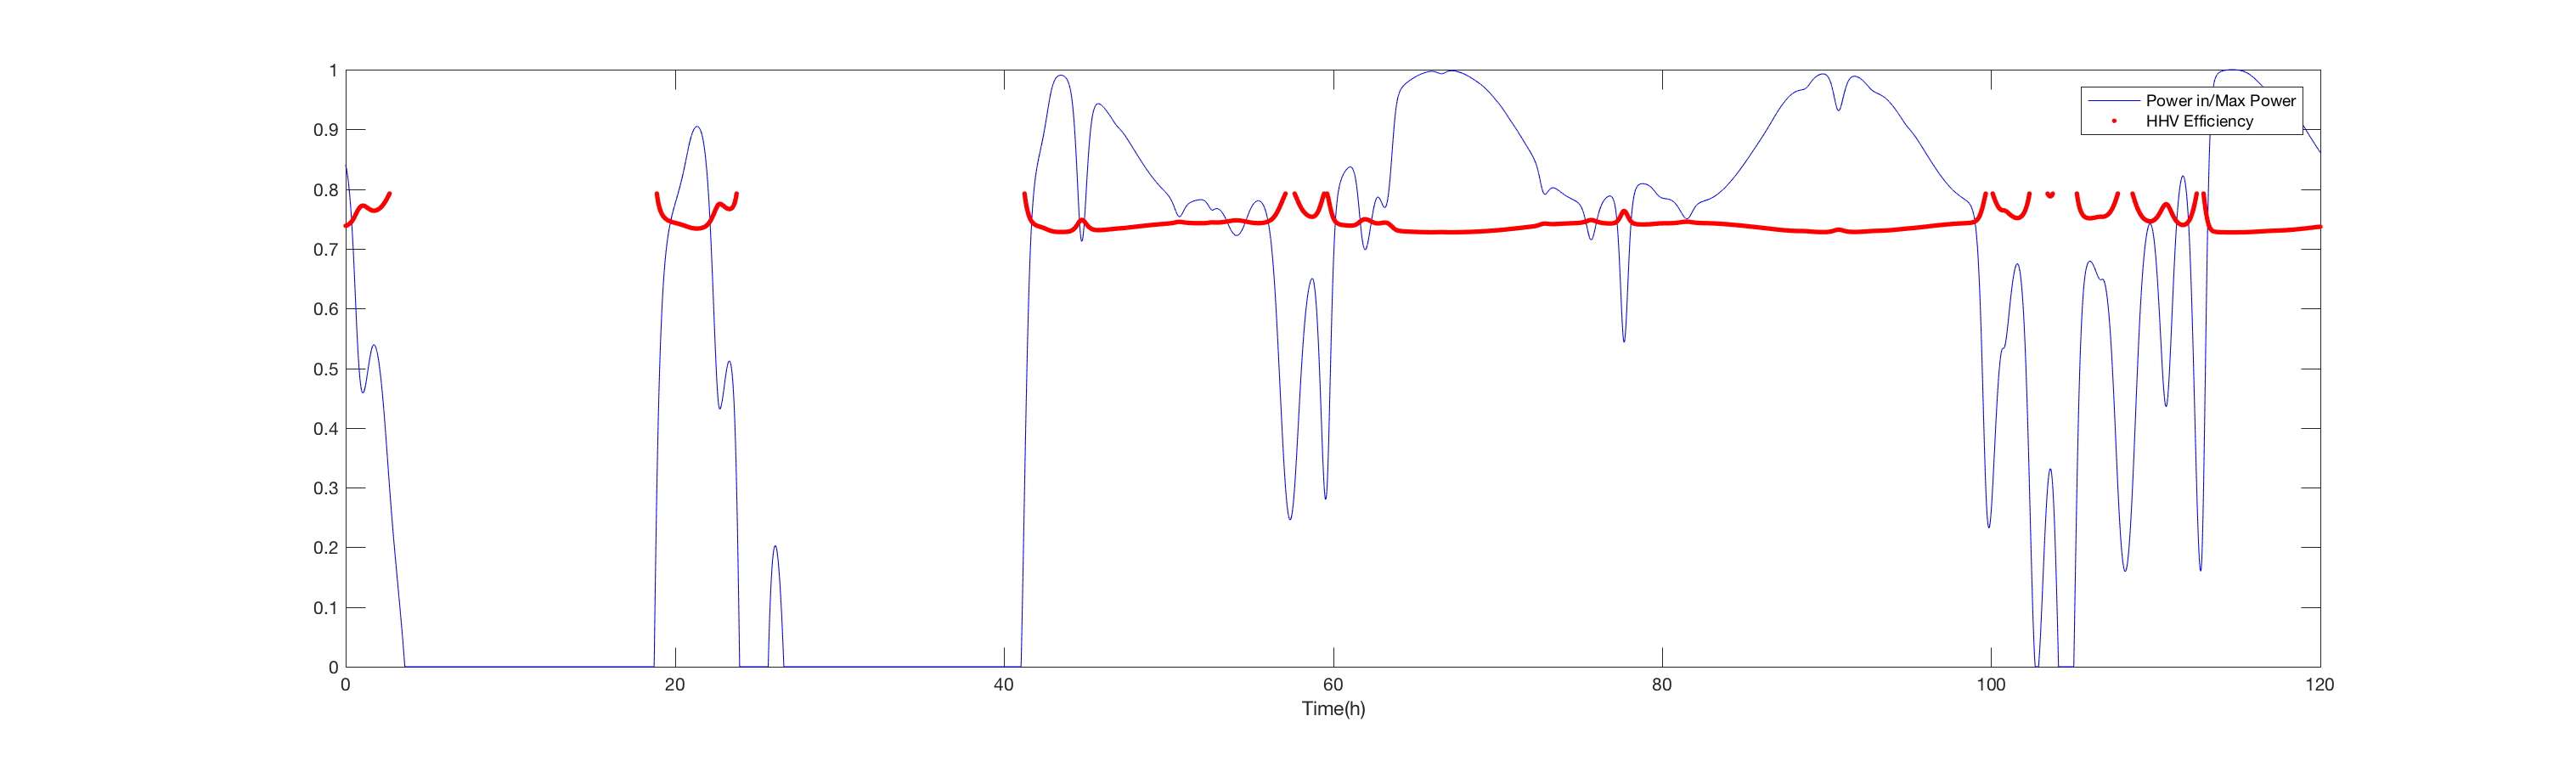
\includegraphics[width=1.0\textwidth]{simulation.eps}
\caption{System Simulation Results[Slide 27]} 
\end{figure} 

\subsection{Summary}
\begin{figure}[H]
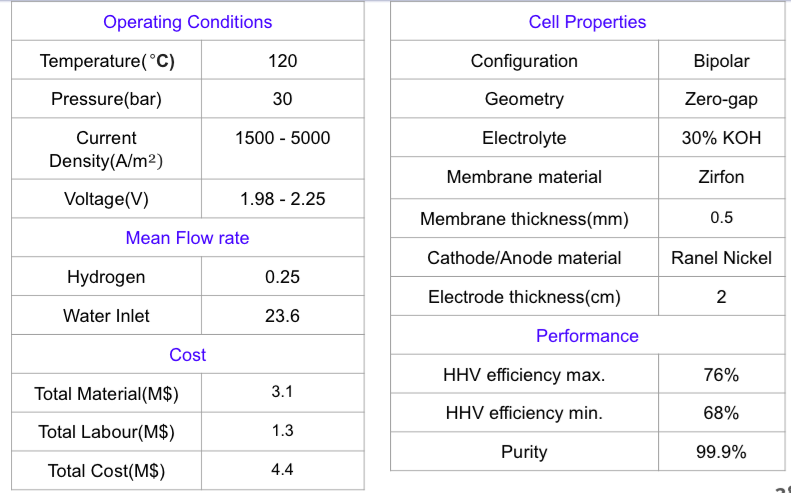
\includegraphics[width=0.99\textwidth]{summary.png}
\caption{Summary of cell properties[Slide 28]}
%\caption{Monopolar and Bipolar configuration[Slide 22]} 
\end{figure} 

